% !TeX root = ..\..\main.tex
\newcommand{\mek}{\mathit{mek}}
\newcommand{\mdk}{\mathit{mdk}}
\newcommand{\id}{\mathit{id}}
%Pseudocode
\begin{itemize}
    \item $\gen\tor(\mek, \mdk)$
    \item $\enc(\mek, \id)\tor(k,c)$
    \item $\del(\mdk, \id)\to\dk_{\id}$
    \item $\dec(\dk_{\id'}, c)\tor k$ iff $\id' = \id$
\end{itemize}

%types of IBE
\begin{tabular}{l p{6cm}}
Standard:&
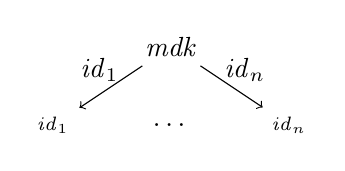
\begin{tikzpicture}[level distance=1cm, baseline=(R.base)] 
    \node (R) at (0,0) {$\mdk$}
        %place child node and use "edge from parent" to place text on the edge
        child[->] {node {$\dk_{\id_1}$} edge from parent node[left=1mm, pos=.1]{$\id_1$}}  
        child {node {\dots} edge from parent[draw=none]}
        child[->] {node {$\dk_{\id_n}$} edge from parent node[right=1mm, pos=.1]{$\id_n$}};
\end{tikzpicture}\\
Hierarchical:&
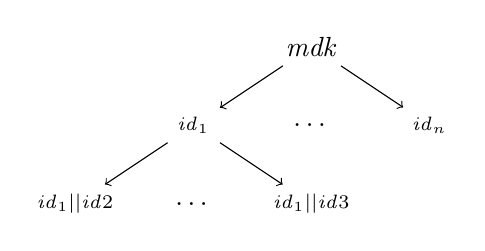
\begin{tikzpicture}[level distance=1cm, baseline=(R.base)] 
    \node (R) at (0,0) {$\mdk$}
        child[->] {node {$\dk_{\id_1}$}
            child[->] {node {$\dk_{\id_1||\id2}$}}
            child {node {\dots} edge from parent[draw=none]}
            child[->] {node {$\dk_{\id_1||\id3}$}}}
        child {node {\dots} edge from parent[draw=none]}
        child[->] {node {$\dk_{\id_n}$}};
\end{tikzpicture}\\
Attribute Based:&
Abstract attributes determine decryptability instead of fixed identities.
\end{tabular}
